\documentclass[12pt,twocolumn]{article}
\usepackage[utf8x]{inputenc}
\usepackage[spanish, es-tabla]{babel}
\usepackage{graphicx}

\usepackage{amsmath}

\title{Proyecto Final}
\author{Juan B. Benavides y Juan P. Vanegas }
\date{\today}

\begin{document}
\maketitle

\section{\label{sec: Intro} Sistema Físico}
La entropía es uno de los conceptos físicos más difíciles de comprender. Para llegar a 
él se puede ver desde el punto de vista termodinámico, o desde un punto de vista más 
cercano a la teoría de la información. A partir de este segundo camino podemos definir la 
entropía como 

\section{Algoritmos y \\ Validación}

Para modelar este fenómeno utilizamos dos paradigmas de programación diferentes: Procedimental 
y Orientado a Objetos, cada uno utilizando un algoritmo de propagación diferente. El 
algoritmo utilizado para el paradigma procedimental, descrito en la figura 
\ref{fig:algoritmo_Proc}, que consta en 
\\
\begin{figure*}
    \centering
    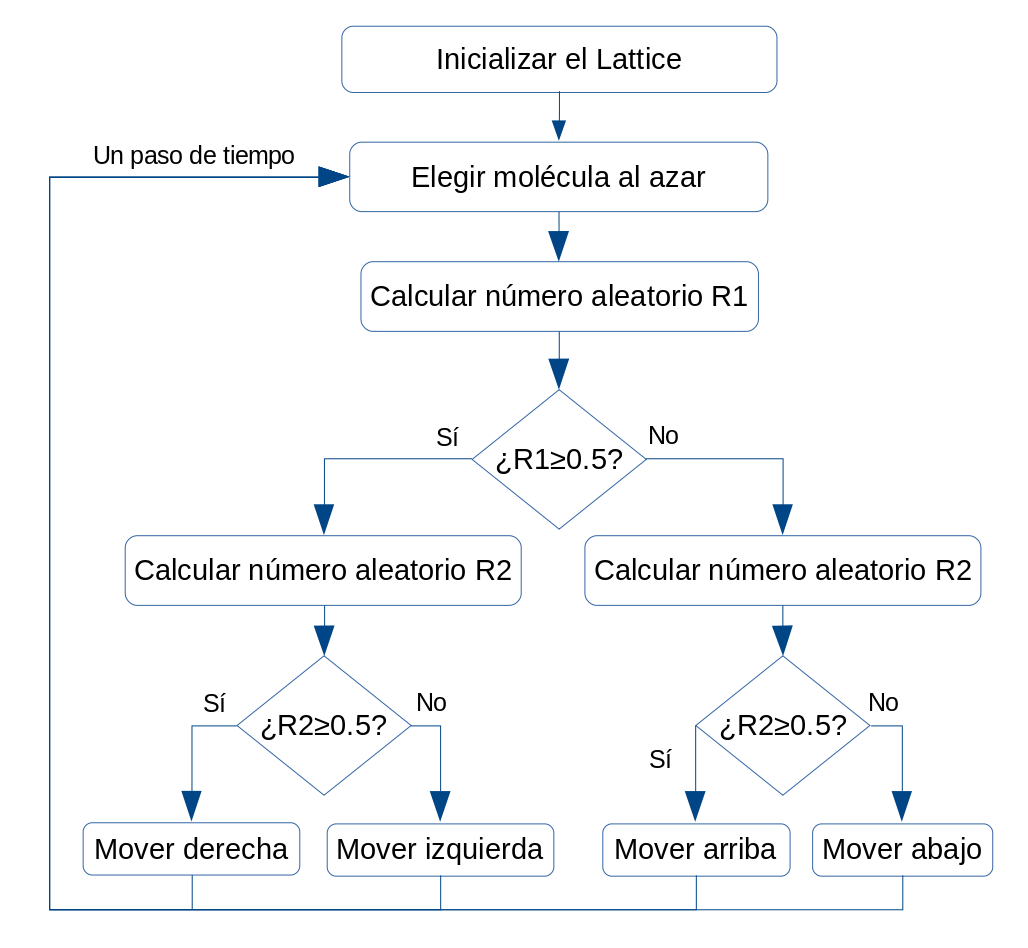
\includegraphics[width=0.75\textwidth]{figs/Algoritmo_Proc.png}
    \caption{Algoritmo 1.}
    \label{fig:algoritmo_Proc}
\end{figure*}

Por otro lado, para el paradigma orientado a objetos se implementó el algoritmo descrito 
en la figura \ref{fig:algoritmo_OOP}, que consiste en una matriz bidimesional de enteros no 
negativos, o Lattice, donde se representan las moléculas como el número de cada celda. Para 
mover las moléculas se recorre el Lattice celda por celda, y en caso de que se encuentre al 
menos una molécula en una celda se mueve a alguna casilla inmediatamente adyacente a la celda. 
Utilizando este algoritmo se toma un paso de tiempo está dado por un recorrido completo al 
Lattice, a diferencia del criterio empleado en el paradigma procedimental. 
\\

Dos factores a considerar en este algoritmo es que, primero, en dado caso que una molécula 
al desplazarse se ubique en la celda donde el algoritmo continúa buscando, esta se moverá 
dos veces. Este caso, aunque poco probable, conlleva a una ligera pérdida de información 
frente al algoritmo procedimental. 
\\

En segundo lugar, dado que un paso de tiempo del paradigma orientado a objetos implica 
mover aproximadamente todas las moléculas, cada paso de tiempo de este algoritmo es N veces 
más rápido que el algoritmo procedural, con N el número inicial de moléculas. Por lo tanto, 
cualquier cálculo que se realize en función del tiempo se verá directamente afectado, 
resultando en que el algoritmo orientado a objetos solo calcula una variable cada 400 
cálculos del algoritmo procedural. Este factor sí debe tenerse en cuenta, y solo puede 
ser despreciado en caso de que el tiempo computacional total que se deba utilizar para 
hallar resultados concluyentes sea mucho mayor a 400.
\\
\begin{figure*}
    \centering
    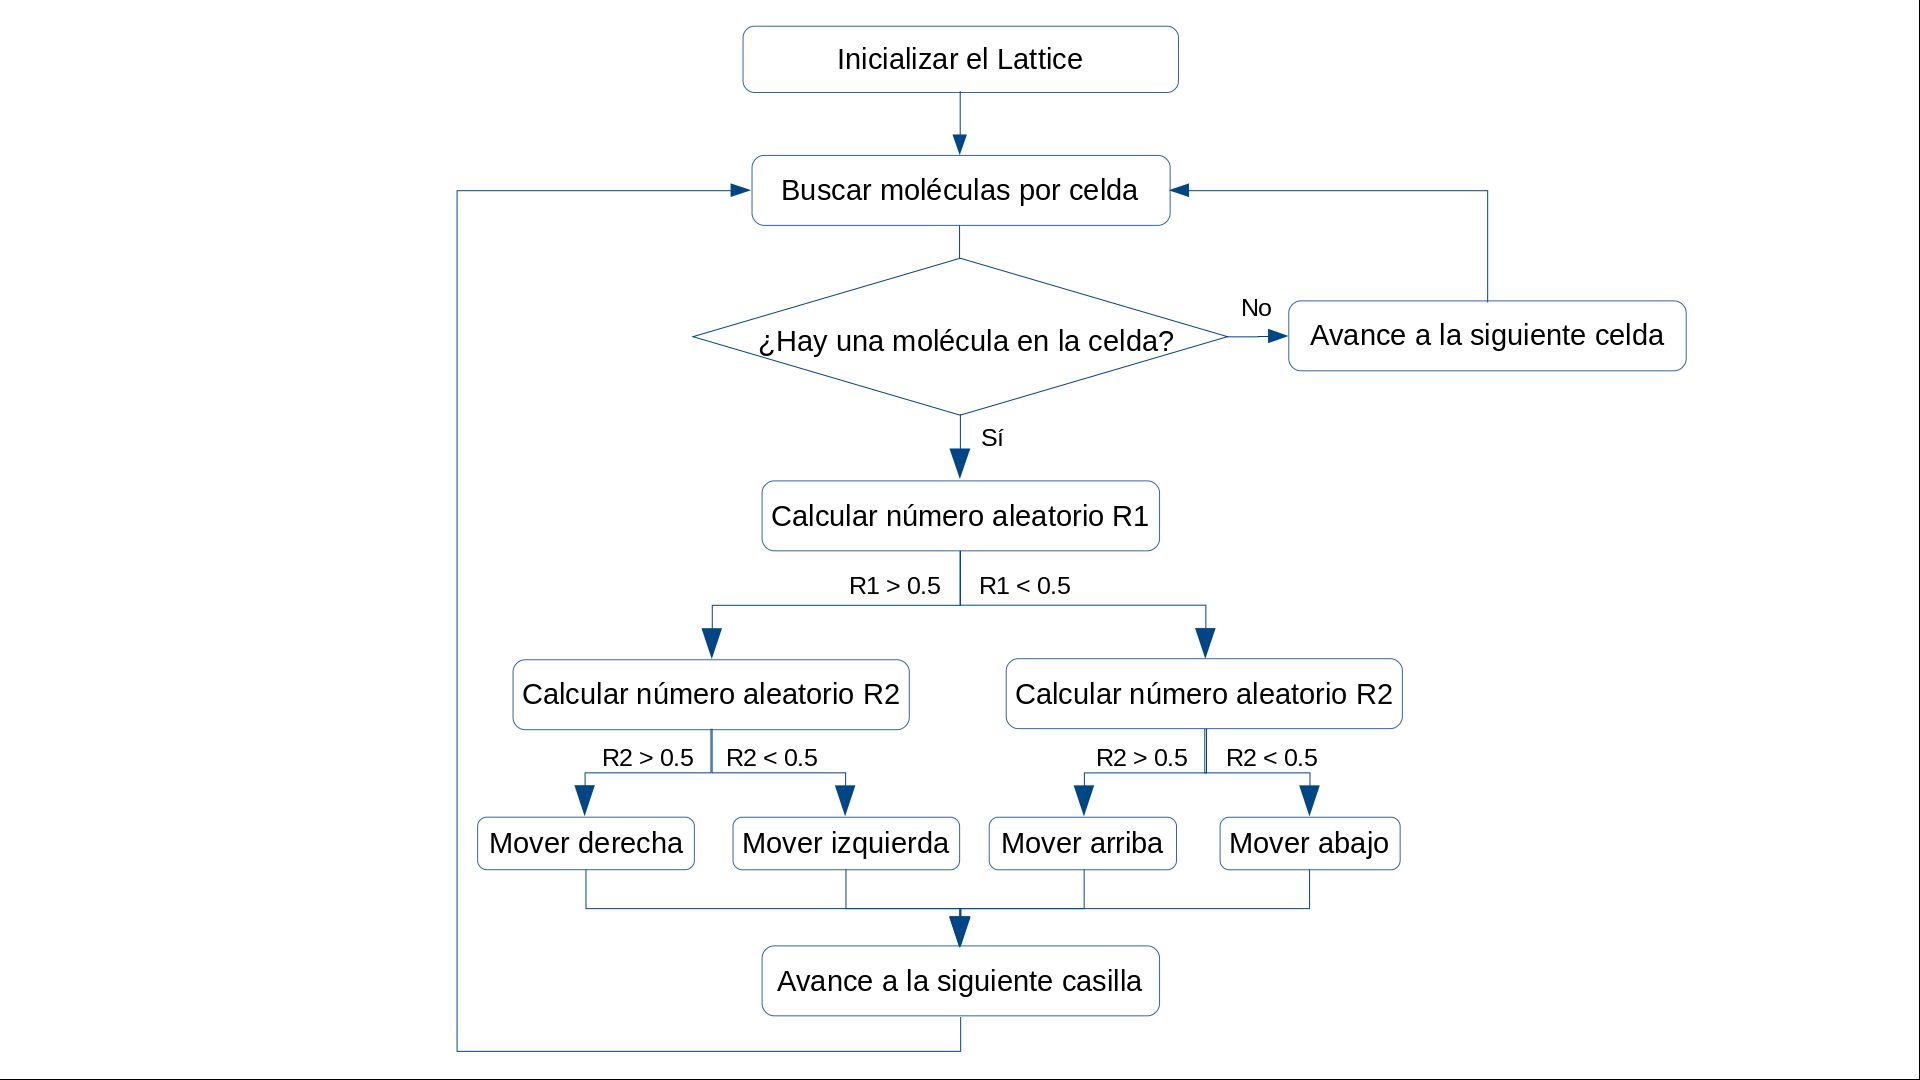
\includegraphics[width=0.75\textwidth]{figs/Algoritmo_OOP.png}
    \caption{Algoritmo 2.}
    \label{fig:algoritmo_OOP}
\end{figure*}

Para validar cada uno de estos métodos se calculó la entropía en función del tiempo de 
cómputo, donde esperamos que inicialmente halla un crecimiento muy rápido de la entropía del 
sistema, que para este caso corresponde a la gota de crema difundiéndose por la taza. Luego 
esperamos que la entropía se estabilice y tenga un comportamiento asintótico alrededor de 
algún valor, que corresponde al momento en el que la crema se halla distribuido de manera 
más o menos uniforme alrededor de la taza.
\\
\begin{figure*}
    \centering
    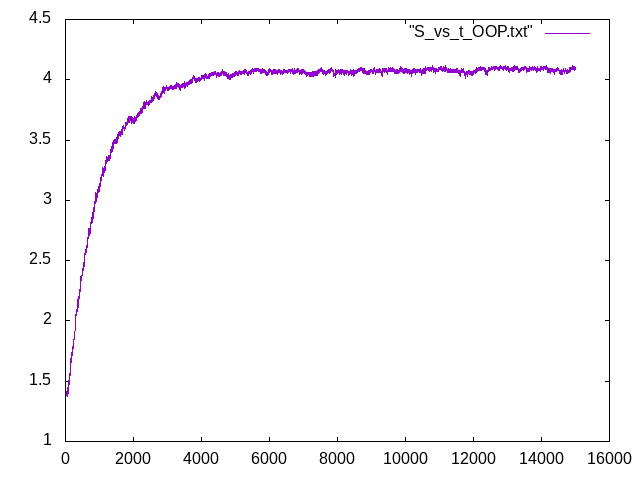
\includegraphics[width=0.75\textwidth]{figs/S_vs_t_OOP.png}
    \caption{Entropía en función del tiempo para paradigma orientado a objetos.}
    \label{fig:s_vs_t_OOP}
\end{figure*}
\begin{figure*}
    \centering
    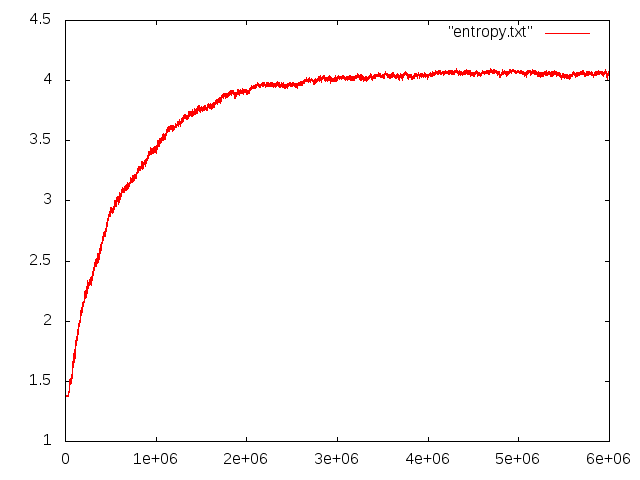
\includegraphics[width=0.75\textwidth]{figs/entropy.png}
    \caption{Entropía en función del tiempo para paradigma procedimental.}
    \label{fig:s_vs_t_Proc}
\end{figure*}

Vemos que en ambos paradigmas, y por lo tanto, algoritmos, el comportamiento de la entropía 
en función del tiempo es el esperado, por lo que ambos métodos quedan validados para modelar 
este sistema. Vemos también que el tiempo de computo total empleado para el paradigma orientado 
a objetos es mucho mayor a 400, con lo que también podemos despreciar la información perdida 
por utilizar este método. A partir de este punto se transformará el tiempo del paradigma 
orientado a objetos multiplicando el tiempo de cómputo por un factor de 400, lo que permite 
comparar directamente los resultados obtenidos en ambos paradigmas.

\section{Resultados y Análisis}

\begin{figure*}
    \centering
    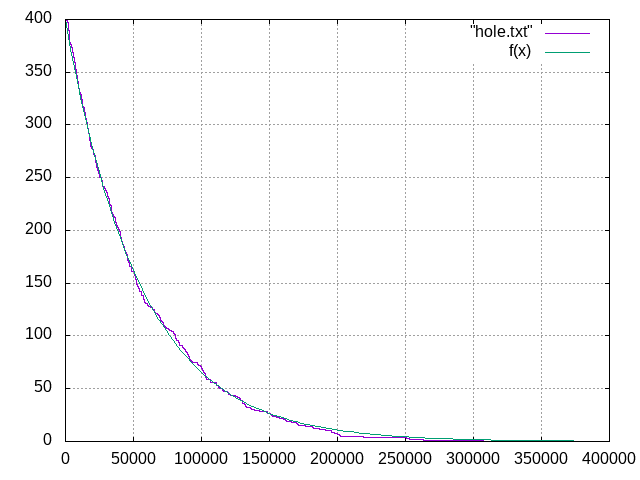
\includegraphics[width=0.75\textwidth]{figs/hole.png}
    \caption{Propagación de las moléculas con un agujero en la pared.}
    \label{fig:hole}
\end{figure*}




\section{Conclusiones}

\end{document}